\documentclass[11pt,letterpaper]{article}
\usepackage{cogsys}
\usepackage{cogsysapa}
% \usepackage{apacite}
% \usepackage{graphicx}
\usepackage[T1]{fontenc}
\usepackage{times}
\usepackage[pdftex]{graphicx} % use this when importing PDF files


% Put back in

 % First page headings for accepted submissions.
% \cogsysheading{1}{2012}{1-18}{9/2012}{12/2012}
 % First page headings for poster submissions.
%\cogsysposterheading{First}{2012}{1-18}

% \ShortHeadings{Formatting Instructions}
              % {P.\ Langley, G.\ Hunt, and D.\ G.\ Shapiro}

\begin{document} 

\title{CDSR Human Data/Modelling Paper}
 
% \author{Pat Langley}{langley@asu.edu}
% \author{Glen Hunt}{glen.hunt@asu.edu}
% \address{Computing Science and Engineering, Arizona State University, 
%          Tempe, AZ 85287 USA}
% \author{Daniel G.\ Shapiro}{dgs@isle.org}
% \address{Institute for the Study of Learning and Expertise, 
%          2164 Staunton Court, Palo Alto, CA 94306 USA}
\vskip 0.2in
 
\begin{abstract}
Representing and reasoning about spatial terms is an essential ability for cognitive systems interacting with humans in a shared environment.  Consider a safe area in a military engagement.  The size, shape, and location of this area depend the the capabilities of the other agents and their capabilities in the environment.  We call these regions \textit{context-dependent spatial regions}(CDSRs).  We claim that understanding these regions requires integrating semantic and geometric knowledge about a dynamic environment.  We conducted a human study to explore how people interpret three types of CDSRs that supports the knowledge integration claim.  We evaluate two representation techniques against the human data and discuss their limitations as a cognitive systems solution to this problem.
\end{abstract}

\section{Introduction - KLENK} 
Natural communication between humans and cognitive systems requires both participants to communicate with spatial language.  Many spatial terms are defined not only be their geometry, but also their context.  That is, to understand this language requires considering the other objects and agents in the environment, as well as their configuration and functional roles.  We call such regions \textit{context-dependent spatial regions}(CDSRs).

We begin by discussing CDSRs with examples.  We claim that (1) people can effectively communicate with these regions, and (2) the size and shape of these regions change with the context.  Next, we discuss desired properties of a cognitive system solution.  The contribution of this paper is a human study exploring our claims about CDSRs and an empirical exploration of current models and their shortcomings.  We close with a discussion of related and future work. 

\section{Context-Dependent Spatial Regions - KLENK}
Consider the following regions (shown in Figure \ref{examples}): the front of a classroom (\ref{fig:classroom}), safety in military engagement (\ref{fig:safety}), or the geographical feature of a bottleneck (\ref{fig:bottleneck}).  To identify these regions, one must identify the physical boundaries (e.g., walls), the objects within the room and their functional use (e.g., desks oriented toward a whiteboard), and other agent's intentions and capabilities (e.g., enemy tanks can move and have a range of attack).  Furthermore, these regions exists at different levels of spatial resolution.  Consider a neighborhood in a city, whose boundaries expand and contract overtime with changes to the surrounding residents and businesses.

%Combine these figures into a single figure across
\begin{figure}
  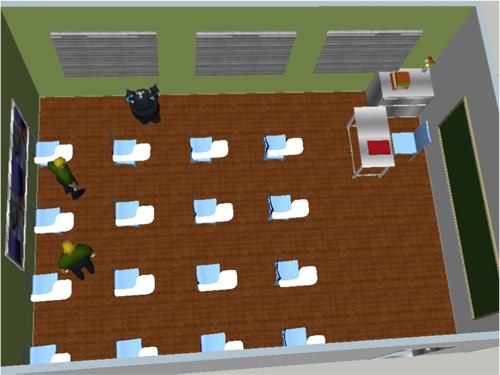
\includegraphics[width=\columnwidth*.3]{figures/classroom.png}
  \caption{The front of the classroom is the area between the desks and the whiteboard where people give presentations.}
  \label{fig:classroom}
\end{figure}

\begin{figure}
  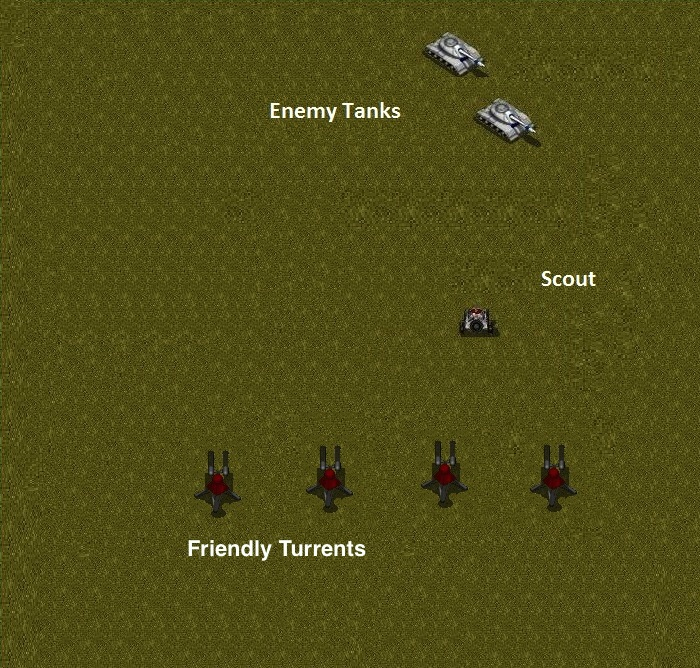
\includegraphics[width=\columnwidth*.3]{figures/safety-3.jpg}
  \caption{Safety for the scout is defined by the location of the friendly turrets and the capabilities of the opposing force.}
  \label{fig:safety}
\end{figure}

\begin{figure}
  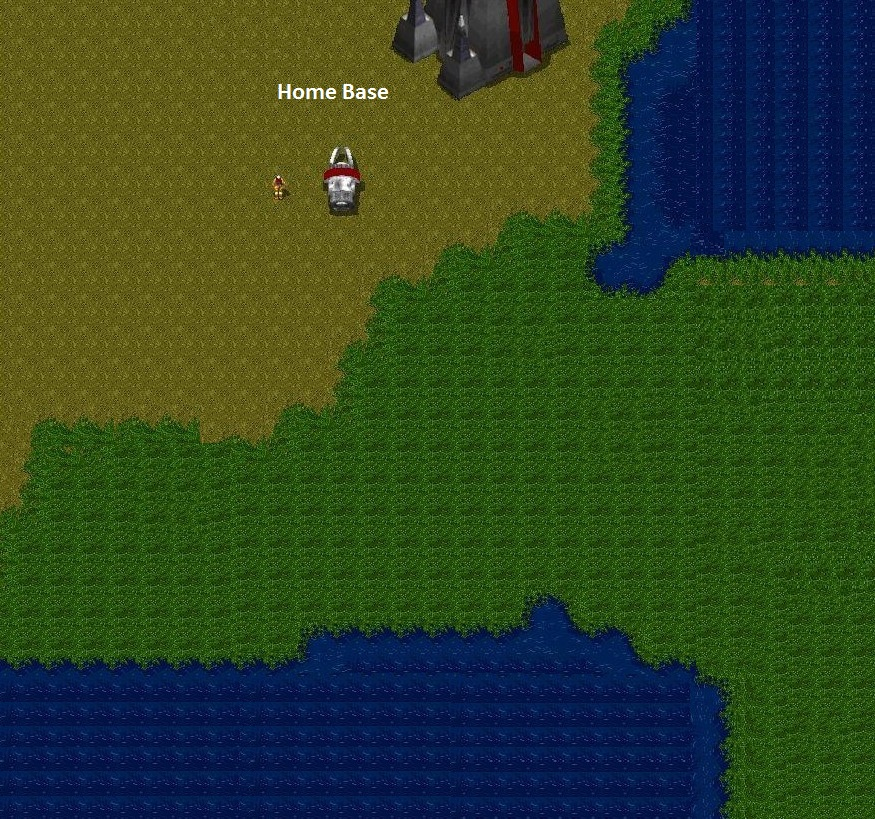
\includegraphics[width=\columnwidth*.3]{figures/bottleneck.JPG}
  \caption{A bottleneck occurs when paths are confined to a narrow region by geographic features.  In this case, the water prevents ground movement.}
  \label{fig:safety}
\end{figure}

Understanding these regions is crucial to joint intelligent action with humans.  Not only are these regions frequently tied to goals and commands: "go to the front of the classroom", "defend the bottleneck", and "get to safety", but they are also central to understanding human activities: e.g., "Is there a class in session?".

Representing and reasoning about these regions is a Cognitive Systems problem. for the following reasons:
\begin{itemize}
\item Understanding context requires integration of different types of knowledge including geometric, semantic, and functional knowledge about the environment.
\item The representation should be transferable to new situations.  While humans do not demonstrate mastery after a single example of concept, they are able to begin using it immediately refining it over time.
\item The representation should be applicable in different reasoning tasks.  The functional nature of these regions makes them important for many tasks from action planning to activity recognition.
\end{itemize}
 
 

\section{Human Studies - John}
Research Questions: 
\begin{enumerate}
	\item Does context matter?
	\item Do people agree? 
\end{enumerate}

Method and Materials 
Trial 1
Trial 2
Trial 3

-----------------

Task 1: The participant draws a polygon denoting the region
Analysis of results:
(1) Do participants agree/understand-the-task? (validation of approach) + Should anyone be excluded?
Within the data for each trial,
-- For each participant, generate the intersection and union polygon of all the other participants
---- Generate N random points in the area of the full stimulus
---- For each of these N points check whether the participant's polygon and the [intersection/union] polygon both include it (agree++) or if one includes it and the other doesn't (disagree++)
---- Then we calculate a Cohen Kappa score as a measure of agreement between the participant and eveyone else. Note we need to calculate the chance of random agreement but we can do this as a function over the relative size of the participant's polygon in the total area of the stimulus and the relative size of the intersection/union polygon
(see http://en.wikipedia.org/wiki/Cohen%27s_kappa )

This process will result in for each trial a list of kappa scores for each participant indicating the extent to which they agree with everyone else. We are hoping for a high kappa score

(2) Does context matter?
I understand that all the rooms stimuli have the same extent.
So one way of evaluating whether context matters is to use the kapp score between the intersection/union polygon generated using all the response (less the excluded partitipants) for one trial and the equivalent polygon for another trial.
We are hoping for a low kappa score

-----------------

Task 2: The participant selected a point denoting the sweetspot of the region
Analysis of results:
(1) Do participants agree/understand-the-task? (validation of approach) + Should anyone be excluded?
Compare the variance across the subjects with the variance across a number of set of randomly generate points, where set size equals the number of participants, using the F distribution (http://www.ltcconline.net/greenl/courses/201/regression/comparingVariances.htm) where we are checking if the variance of the random points are greater than that of the participants.
We would hope that the variance of the subjects responses is lower than that of randomly generated points.
After the initial comparison with the random point sets we may exclude participants based on extreme variance.
 
(2) Does context matter?
Do the clusters of participants responses move?
- for each experimental stimulus compute the mean x and y location for the responses for that trial
- check whether the variance between the means of different stimuli responses is greater than the variance within each stimulus responses.

-----------------


Task 3: The participant grades a point with respect to membership of the region on a likert scale
I understand this experiment to be useful because (a) it asks the participants to evaluate (rather than generate cf task 1 and 2) (b) hopefully we can use it to reinforce our findings in task 1 and task 2
I think we need to be careful that the points we present to people for evaluation are reasonably well distributed so that we have a good chance of getting a variation across the responses
Assuming that there is a variation across the likert scores for a particular stimulus then check if their is a correlation between the scores and:
(a) inclusion in the intersection/union polygons from task 1 for the same stimulus
(b) distance from the mean sweet spot for that stimulus from task 2

-----------------
 




\section{Modeling - Nick}


As the results above show, in order for an artificial cognitive system to operate successfully with humans (e.g. understanding spatially-situated task utterances), they must have access to internal models which can represent CDSRs and recognise them in new environments. Whilst spatial reasoning has been an active topic in AI and robotics for decades, CDSRs present a new problem which requires solutions beyond the current state-of-the-art. Regions are central to QSR work~\cite{Cohn:2001}. Regions can either have crisp boundaries, usually defined by geometric shapes (e.g. the bounding boxes of visually tracked objects~\cite{SridharCohn:10}), or vague boundaries created qualitatively by multiple crisp regions (e.g. the `egg-yolk model'~\cite{Cohn96b}), or by thresholding an underlying spatially-mapped function (e.g. those created by potential fields~\cite{brenneretal07ijcai} or by Gaussian kernels~\cite{burbridge-dearden12}). The fundamental decision when creating a computational model of a CDSR is the method used to represent its boundary. Given their context-dependent nature, boundary definitions based purely on single geometric shapes seem unlikely to work. However, arbitrary boundaries can be defined using a sequence of geometric primitives (usually straight lines), as in chain code for image region representations~\cite{Freeman:1961}. This is an approach we followed in previous work, where boundary segments connected vertices defined by contextually-appropriate anchor points~\cite{Hawes:2012}.  Whilst our previous approach provided basic performance, the crisp boundaries it generated caused mismatches with human data over the extent of regions. Methods based on underlying spatial functions may be more flexible in this regard, as they can be selectively thresholded depending on context. 

% Basic approaches

\textbf{TODO:} Perhaps add related work on robot spatial representations, e.g. maps, rooms.  

In the following sections we explore whether two possible CDSR models (one based on boundary segments, one based on a spatial function) are able to satisfy the previously described desiderata for a cognitive systems approach to representing and recognising CDSRs. The surrounding discussion is intended to explore the strengths and weaknesses of these models, providing directions for future research.

\subsection{Symbolic Boundary Method - KLENK}
In our previous work \cite{Hawes:2012}, we presented an approach on a mobile robot that combined qualitative spatial relations, object recognition, and analogy to transfer CDSRs represented as polygons defined by \textit{anchor points} \cite{DBLP:journals/jetai/KlenkFTK11}.  Anchor points are symbolic descriptions that link a conceptual entity (e.g., the front of a classroom) to perceived entities (e.g., the lower left extent of a desk).  An example of the representation and transfer approach is Figure \ref{fig:anchor-point-transfer}.  In the know example, a human defines the front of the classroom as a polygon consisting of four anchor points.  Analogical transfer works by aligning structured representations and transferring partially aligned statements from the known example to the new environment.  In this case, the anchor points are transferred from the group of desks in the known example to the corresponding group of desks in the new environment. 

\begin{figure}
  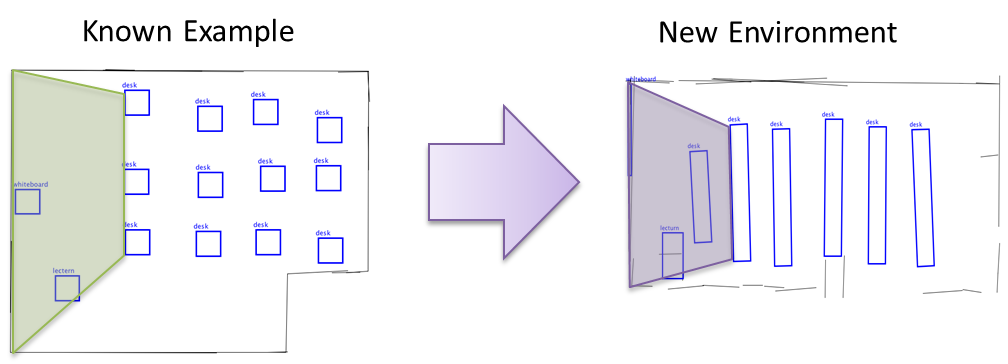
\includegraphics[width=\columnwidth]{figures/classroom-transfer.png}
  \caption{The known example defines the front of the room with four anchor points.  By transferring the anchor points to the new environment, the system is able to ground the room's front in its perception.}
  \label{fig:anchor-point-transfer}
\end{figure}

This method satisfies our criteria for a cognitive systems solution for the following reasons: (1) the alignment process integrates spatial and semantic knowledge about the environment, (2) analogy enables transfer from a single example, (3) while untested, by linking conceptual knowledge to perception, regions defined by anchor points should support any symbolic reasoning task.
 
Applying this model to the points and regions indicated in our experiment illustrates two limitations.  Regions do not always physically bounded by objects.  In the classroom examples, people frequently did not extend the front of the room all way into the corners.  In the safety example, people did not indicate that it was safe behind the lone turret in front of the others.  This indicates that people consider the dynamics of the situation when evaluating these terms, which is not accounted for in this model.

\subsection{Spatial Function Method - NICK}

Overview - either Chris's approach or something similar
Example
Results?
Discussion 
Where do the points come from

\section{Discussion}
 
\begin{acknowledgements} 
\noindent
STRANDS etc.
\end{acknowledgements} 




\vspace{-0.25in}

{\parindent -10pt\leftskip 10pt\noindent
\bibliographystyle{cogsysapa}
\bibliography{cdsr}

}

% Leave a blank line before the closing brace to ensure the final 
% reference has the proper indentation. 

\end{document} 
